% \documentclass[12pt]{article}
%  \usepackage[margin=1in]{geometry}
% \usepackage{amsmath, amsthm, amssymb, amsfonts, enumitem, fancyhdr, color, comment, graphicx, environ, fancyhdr}
% \pagestyle{fancy}
% \usepackage{cmap}
% \usepackage[T2A]{fontenc}
% \usepackage[utf8]{inputenc}
% \usepackage[english, russian]{babel}
% \usepackage{caption}
%
% \newtheorem*{exersize}{Упражнение}
% \newtheorem*{lemma}{Лемма}
% \newtheorem*{theorem}{Теорема}
% \newtheorem*{consequence}{Следствие}
% \newtheorem*{statement}{Утверждение}
% \newtheorem{property}{Свойство}
% \newtheorem*{fact}{Факт}
%
% \theoremstyle{definition}
% \newtheorem*{definition}{Определение}
% \newtheorem*{problem}{Задача}
% \newtheorem*{example}{Пример}
%
% \theoremstyle{remark}
% \newtheorem*{note}{Замечание}
% \setlength{\parindent}{0pt}
% \setlength{\headheight}{35pt}
%
%
% \begin{document}

\section{Динамические модели}
\subsection{Модель Солоу}
Пусть имеется замкнутая односекторная экономика.\\
$Y$ - ВВП\\
$K$ - капитал\\
$I$ - инвестиции\\
$C$ - конечное потребление\\
$L$ - трудовые ресурсы\\
Имеется баланс $Y=C+I$. Зависимость ВВП от ресурсов выражается функцией Кобба-Дугласа.
\begin{align}
  &Y=AK^{\alpha}L^{\beta}\notag\\
  &Y=C+I\notag\\
  &I=sY\\
  &\dfrac{\partial L}{\partial t}=\gamma L \qquad \qquad\quad\,(L(0)=L_0)\notag\\
  &\dfrac{\partial K}{\partial t}=-\mu K+I \qquad(K(0)=K_0)\notag
\end{align}
где $ \gamma$ - темп прироста трудовых ресурсов, $s$ - склонность к сбережению, $A$ - научно-технический прогресс.
Пусть $y=Y/L,k=K/L,i=I/L$. Тогда получим модель Солоу в относительных показателях.
\begin{equation}
  \frac{\partial k}{\partial t}=-(\lambda+\mu)k+sAk^{\alpha}
\end{equation}
Равновесие равно $\hat{k}=(\dfrac{sA}{\lambda+\mu})^{\frac{1}{1-\alpha}}$
\begin{center}
\begin{tabular}{|c|c|}
  \hline
  Интервалы&Рост\\
  \hline
  $\bigg(0;(\dfrac{\alpha sA}{\lambda+\mu})^{\frac{1}{1-\alpha}}\bigg)$&Ускоренный рост\\
  \hline
  $\bigg((\dfrac{\alpha sA}{\lambda+\mu})^{\frac{1}{1-\alpha}};(\dfrac{sA}{\lambda+\mu})^{\frac{1}{1-\alpha}}\bigg)$&Насыщенный рост\\
  \hline
  $\bigg((\dfrac{sA}{\lambda+\mu})^{\frac{1}{1-\alpha}};+\infty\bigg)$&Падение\\
  \hline
\end{tabular}
\end{center}
\textbf{Конечно-разностное представление}:
$k(t+\Delta)=k(t)+\Delta t(-(\lambda+\mu)k(t)+sAk(t)^{\alpha})$
На рисунке 6 показана реализация модели Солоу на Python. На графике представлены три решения с разными задачами Коши. Также при помощи горизонтальных прямых график разбит на интервалы, описанные раннее.
Для численного решение здесь и далее используется метод численного решения обыкновенных дифференциальных уравнений Рунге-Кутта порядка 4 (рис. 7).
\begin{center}
  \begin{tabular}{c}
    \includegraphics[scale=0.6]{images/solow.png}\\
    Рисунок 6 - Модель Солоу\\
    \includegraphics[scale=0.6]{images/R-K.png}\\
    Рисунок 7 - Метод Рунге-Кутта
  \end{tabular}
\end{center}


\subsection{SIR модель}
Пусть $S(t)$ - число восприимчивых к инфекции\\
$I(t)$ - число инфицированных\\
$R(t)$ - число переболевших инфекцией\\
$N$ - число популяции\\
$\beta$ - коэффициент интенсивности контактов \\
$\gamma$ - коэффициент интенсивности выздоровления
\begin{align}
  &\dfrac{d S}{dt}=\dfrac{-\beta IS}{N}\notag\\
  &\dfrac{d I}{dt}=\dfrac{\beta IS}{N}-\gamma I\\
  &\dfrac{d R}{dt}=\gamma I\notag
\end{align}

Далее представлена реализация данной модели в среде AnyLogic. На рисунке 8 показана модель при $\beta=3/14,\gamma=1/14 $, где знаменатель это среднее время выздоровления. По данной модели видно, что сперва идет рост инфицированных, затем он доходит до своего пика (за этот пик отвечают параметры  $\beta,\gamma$). После пика начинается спад и спустя какое-то время видна стабилизация, скорость выздоровления начинается снижаться, так как после пика распространение эпидемии сокращается.
\begin{center}
  \begin{tabular}{c}
    \includegraphics[scale=0.5]{images/sir(1).png}\\
    Рисунок 8 - SIR модель ($\beta=3/14,\gamma=1/14 $)
  \end{tabular}
\end{center}

На рисунке 9 представлена SIR модель с увеличенным параметров $\beta$. Как видно при его увеличении пик распространения эпидемии наступает намного быстрее, что соответствует если в действительности увеличить число контактов.
\begin{center}
  \begin{tabular}{c}
    \includegraphics[scale=0.5]{images/sir(2).png}\\
    Рисунок 9 - SIR модель с увеличенным $\beta$
  \end{tabular}
\end{center}

На рисунке 10 увеличен параметр $\gamma$ - коэффициент интенсивности выздоровления. Увеличивая его, люди слишком быстро выздоровливают и соответственно пик эпидемии наступает рано и незначителен по своей величине.
\begin{center}
  \begin{tabular}{c}
    \includegraphics[scale=0.5]{images/sir(3).png}\\
    Рисунок 10 - SIR модель с увеличенным $\gamma$
  \end{tabular}
\end{center}

\subsection{SEIRD модель}
$E(t)$ - число носителей заболевания\\
$D$ - число умерших\\
$\mu$ - уровень смертности\\
$\delta=\dfrac{1}{\text{ср.инк.период}}$
\begin{align}
  &\dfrac{d S}{dt}=\dfrac{-\beta IS}{N}\notag\\
  &\dfrac{d E}{dt}=\dfrac{\beta IS}{N}-\delta E\notag\\
  &\dfrac{d I}{dt}=\delta E-\gamma I-\mu I\\
  &\dfrac{d R}{dt}=\gamma I\notag\\
  &\dfrac{d D}{dt}=\mu I\notag
\end{align}

В данной модели в отличие от предыдущий, люди заболевают не сразу, а есть некоторый инкубационный период, то есть сначала они получают статус exposed, а только затем infected. Также в данной модели есть убыль популяции, за счет смертности. На рисунке 11 представлена реализация с введением в SEIRD модель вакцинации. Вакцинация по факту дает возможность перейти из восприимчивого к агенту с иммунитетом, но также есть и вероятность рецидивы, когда вакцина не подействовала.
\begin{center}
  \begin{tabular}{c}
    \includegraphics[scale=0.45]{images/seird (1).png}\\
    Рисунок 11 - SEIRD модель
  \end{tabular}
\end{center}

На рисунке 12 увеличен уровень вакцинации, что приводит к значительному увеличению числа выздоровевших.
\begin{center}
  \begin{tabular}{c}
    \includegraphics[scale=0.45]{images/seird (2).png}\\
    Рисунок 12 - SEIRD модель с увеличенной вакцинацией
  \end{tabular}
\end{center}

На рисунке 13 показана модель при увеличение уровня смертности. В следствии сильное сокращения числа популяции.
\begin{center}
  \begin{tabular}{c}
    \includegraphics[scale=0.45]{images/seird (3).png}\\
    Рисунок 13 - SEIRD модель с увеличенным $\mu$
  \end{tabular}
\end{center}

\subsection{Модель Лотки-Вольтерра}
\begin{equation}
  \begin{cases}
    \dot{x}=ax-bxy\\
    \dot{y}=-cy+dxy
  \end{cases}
\end{equation}
$x(t)$ - число жертв\\
$y(t)$ - число хищников\\
$a$ - коэффициент рождаемости жертв\\
$b$ - коэффициент убыли жертв\\
$c$ - коэффициент убыли хищников \\
$d$ - коэффициент рождаемости хищников\\

Первой стационарной точкой является $(0,0)$. Возьмем из системы линейную часть и составим матрицу.
\begin{equation}
  \begin{vmatrix}
  a-\lambda&0\\0&-c-\lambda\;
\end{vmatrix}
\end{equation}

Решая данной характеристическое уравнение получим $\lambda_1=a, \lambda_2=-c\Rightarrow$ данная точка является седлом.
Теперь приравняем правые части системы к 0 и решим ее. Получим вторую стационарную точку $\overline{x}=\dfrac{c}{d},
\overline{y}=\dfrac{a}{b}$. Построим матрицу Якоби, подставив $\overline{x},\overline{y}$.
\begin{equation}
  \begin{pmatrix}
    0&-\dfrac{bc}{d}\\-\dfrac{ad}{b}&0
  \end{pmatrix}
\end{equation}
Решая характеристическое уравнение $\lambda^2+ac=0$, получаем два мнимых корня, что свидетельствует о том что данная
стационарная точка является центром (рис. 14).
\begin{center}
  \begin{tabular}{c}
    \includegraphics[scale=0.5]{images/lv_1 (2).png}\\
    Рисунок 14 - Состояния равновесия
  \end{tabular}
\end{center}
На рисунке 15 приведена реализации модели Лотки-Вольтерра в AnyLogic.
\begin{center}
  \begin{tabular}{c}
    \includegraphics[scale=0.4]{images/lv_1.png}\\
    Рисунок 15 - Модель Лотки-Вольтерра AnyLogic
  \end{tabular}
\end{center}
На рисунке 16 приведена реализации модели Лотки-Вольтерра на Python.
\begin{center}
  \begin{tabular}{c}
    \includegraphics[scale=0.5]{images/lv_2.png}\\
    Рисунок 16 - Модель Лотки-Вольтерра Python
  \end{tabular}
\end{center}

\subsection{Взаимодействие двух конкурирующих видов}
$x_1$ - количество особей первого типа
$x_2$ - количество особей второго типа
\begin{equation}
  \begin{cases}
    \dot{x}_1=a_1x_1-b_{11}x_1^2-b_{12}x_1x_2\\
    \dot{x}_2=a_2x_2-b_{21}x_1x_2-b_{22}x_2^2
  \end{cases}
\end{equation}
Приравняем к 0 правые части системы.
\begin{equation}
  \begin{cases}
    x_1(a_1-b_{11}x_1-b_{12}x_2)=0\\
    x_2(a_2-b_{21}x_1-b_{22}x_2)=0
  \end{cases}
\end{equation}
Получим 4 стационарные точки.
\begin{gather}
  \begin{cases}
    x_1=0\\
    x_2=0
  \end{cases};
  \begin{cases}
    x_1=0\\
    x_2=\dfrac{a_2}{b_{22}}
  \end{cases};\\
  \begin{cases}
    x_1=\dfrac{a_1}{b_{11}}\\
    x_2=0
  \end{cases};
  \begin{cases}
    x_1=\dfrac{a_2b_{12}-a_1b_{22}}{b_{12}b_{21}-b_{22}b_{11}}\\
    x_2=\dfrac{a_1b_{21}-a_2b_{11}}{b_{12}b_{21}-b_{22}b_{11}}
  \end{cases}\notag
\end{gather}
Определим состояние равновесия для каждой стационарной точки
\begin{enumerate}
  \item 1
  \item 2
\end{enumerate}
Для численного анализа данной модели модифицируем метод Рунге-Кутта для двух функций (рис. 17).
\begin{center}
  \begin{tabular}{c}
    \includegraphics[scale=0.5]{images/tcs (1).png}\\
    Рисунок 17 - Метод Рунге-Кутта для двух функций
  \end{tabular}
\end{center}
На рисунке 18 приведены значения параметров для которых производился расчет.
\begin{center}
  \begin{tabular}{c}
    \includegraphics[scale=0.5]{images/tcs (2).png}\\
    Рисунок 18 - Параметры
  \end{tabular}
\end{center}
На рисунке 19 показано численное решение. Как видно сначала две популяции убывали, но затем вторая начала рост до некоторого равновесного состояния.
\begin{center}
  \begin{tabular}{c}
    \includegraphics[scale=0.45]{images/tcs (3).png}\\
    Рисунок 19 - Два конкурирующих вида
  \end{tabular}
\end{center}
Теперь посмотри на результат в плоскости двух популяций. На рисунке 20 приведен график векторного поля, то есть касательных к интегральной кривой. Здесь видны равновесные состояния описанные ранее. Для точки $(0,0)$ неустойчивый узел, все вектора расходятся от данной точки. Точки $(0,\dfrac{a_2}{b_{22}}),(\dfrac{a_1}{b_{11}},0)$ являются устойчивыми узлами и следовательно к ним вектора сходятся.
\begin{center}
  \begin{tabular}{c}
    \includegraphics[scale=0.45]{images/tcs (4).png}\\
    Рисунок 20 - Два конкурирующих вида
  \end{tabular}
\end{center}
Для того чтобы увидеть 4 точку, которая является седловой обратимся к рисунку 21. Здесь представлен \textit{dashboard} по данной модели и отчетливо видны все 4 точки. Данный график реализован при помощи библиотеки \textit{Plotly}.
\begin{center}
  \begin{tabular}{c}
    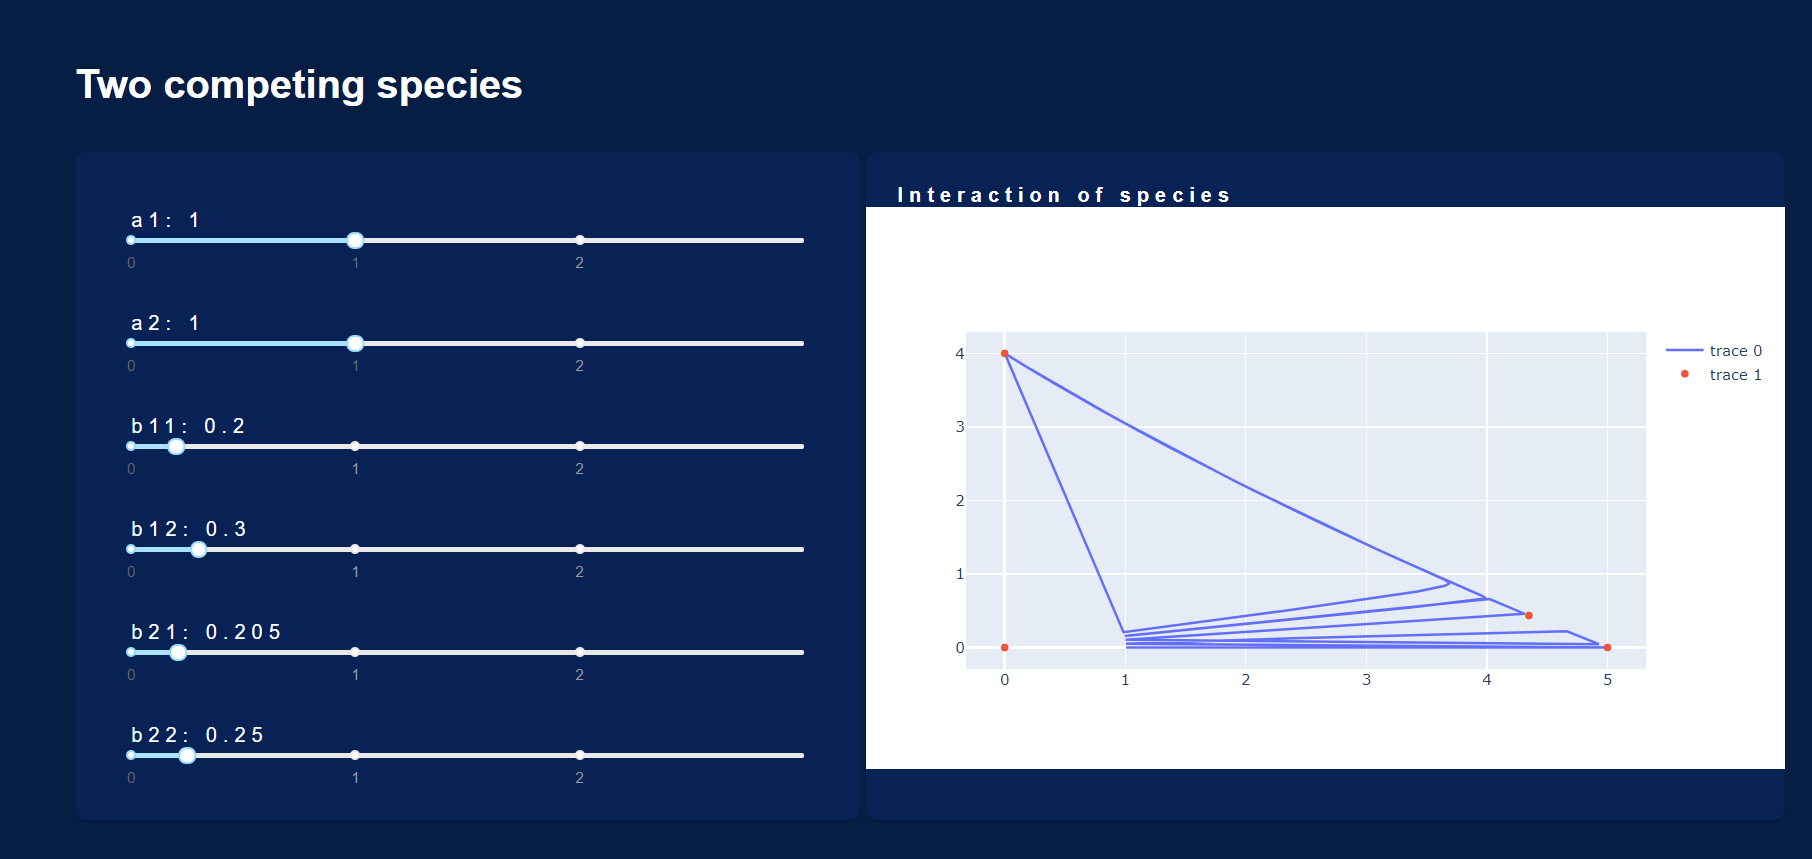
\includegraphics[scale=0.3]{images/Dashboard1.png}\\
    Рисунок 21 - Два конкурирующих вида (dashboard)
  \end{tabular}
\end{center}

\subsection{Переход к полярным координатам}
\begin{equation}
\begin{cases}
  \dot{x}_1=x_1-x_2-x_1(x_1^2+x_2^2)\\
  \dot{x}_2=x_1+x_2-x_2(x_1^2+x_2^2)
\end{cases}
\end{equation}
Перейдем к полярным координатам.
\begin{equation}
  \begin{cases}
    x_1(t)=r(t)\cos{\varphi(t)}\\
    x_2(t)=r(t)\sin{\varphi(t)}
  \end{cases}
\end{equation}
Выполним подстановку и получим выражения для $\dot{r}$ и $\dot{\varphi}$.
\begin{align}
  &\begin{cases}
    \dot{r}\cos{\varphi}+r\dot{\varphi}(-\sin{\varphi})=r\cos{\varphi}-r\sin{\varphi}-r^3\cos{\varphi}\;\big|*\cos{\varphi}\\
    \dot{r}\sin{\varphi}+r\dot{\varphi}\cos{\varphi}=r\cos{\varphi}+r\sin{\varphi}-r^3\sin{\varphi}\quad\quad\big|*\sin{\varphi}
  \end{cases}+\\
  &\begin{cases}
    \dot{r}\cos^2{\varphi}-r\dot{\varphi}\sin{\varphi}\cos{\varphi}=
    r\cos^2{\varphi}-r\cos{\varphi}\sin{\varphi}-r^3\cos^2{\varphi}\\
    \dot{r}\sin^2{\varphi}+r\dot{\varphi}\cos{\varphi}\sin{\varphi}=
    r\sin{\varphi}\cos{\varphi}+r\sin^2{\varphi}-r^3\sin^2{\varphi}
  \end{cases}
\end{align}
Тем самым получаем выражение для $\dot{r}(t)=r(t)(1-r^2(t))$. Теперь умножим первое уравнения на $sin{\varphi}$,
второе на $cos{\varphi}$ и вычтем из первого второе.
\begin{align}
  &\begin{cases}
    \dot{r}\cos{\varphi}+r\dot{\varphi}(-\sin{\varphi})=r\cos{\varphi}-r\sin{\varphi}-r^3\cos{\varphi}\;\big|*\sin{\varphi}\\
    \dot{r}\sin{\varphi}+r\dot{\varphi}\cos{\varphi}=r\cos{\varphi}+r\sin{\varphi}-r^3\sin{\varphi}\quad\quad\big|*\cos{\varphi}
  \end{cases}-\\
  &\begin{cases}
    \dot{r}\cos{\varphi}\sin{\varphi}-r\dot{\varphi}\sin^2{\varphi}=
    r\cos{\varphi}\sin{\varphi}-r\sin^2{\varphi}-r^3\cos{\varphi}\sin{\varphi}\\
    \dot{r}\sin{\varphi}\cos{\varphi}+r\dot{\varphi}\cos^2{\varphi}=
    r\cos^2{\varphi}+r\sin{\varphi}\cos{\varphi}-r^3\sin{\varphi}\cos{\varphi}
  \end{cases}
\end{align}
Таким образом получим систему (1) в полярных координатах.
\begin{equation}
  \begin{cases}
    \dot{r}=r(1-r^2)\\
    \dot{\varphi}=1
  \end{cases}
\end{equation}
Стационарные точки для данной системы $r=0$ и $r=1$.\\
Устойчивый предельный цикл (рис. 22):
\begin{equation}
  \begin{cases}
    \dot{r}=r(1-r^2)\\
    \dot{\varphi}=1
  \end{cases}
\end{equation}

\begin{center}
  \begin{tabular}{c}
    \includegraphics[scale=0.4]{images/polar (1).png}\\
    Рисунок 22 - Устойчивый предельный цикл
  \end{tabular}
\end{center}

Неустойчивый предельный цикл (рис. 23):
\begin{equation}
  \begin{cases}
    \dot{r}=r(r^2-1)\\
    \dot{\varphi}=1
  \end{cases}
\end{equation}

\begin{center}
  \begin{tabular}{c}
    \includegraphics[scale=0.4]{images/polar (2).png}\\
    Рисунок 23 - Неустойчивый предельный цикл
  \end{tabular}
\end{center}

Полуустойчивый предельный цикл (рис. 24):
\begin{equation}
  \begin{cases}
    \dot{r}=r(1-r)^2\\
    \dot{\varphi}=1
  \end{cases}
\end{equation}

\begin{center}
  \begin{tabular}{c}
    \includegraphics[scale=0.4]{images/polar (3).png}\\
    Рисунок 24 - Полуустойчивый предельный цикл
  \end{tabular}
\end{center}

\subsection{Модель Самуэльсона-Хикса}
\subsubsection{Дискретная форма}
Предполагается замкнутая экономика, предложение эластично, цены и процентная ставка фиксированы.
Рассмотрим уравнение
\begin{equation}
  Y_{t+1}=C(Y_t)+I_t
\end{equation}
Пусть спрос зависит от $Y_t$ линейно, т.е. $C(Y_t)=C_a+cY_t$, а инвестиции равны $I_t=r(Y_t-Y_{t-1}) +I_a$, где
$C_a$ - постоянное потребление, $I_a$ - постоянные инвестиции, $r$ - коэффициент акселерации, $c$ - склонность к потреблению.
 $A=C_a+I_a$ - автономные расходы. Получим следующее конечно-разностное уравнение.
 \begin{equation}
   Y_{t+1}=C_a+I_a + cY_t + r(Y_t-Y_{t-1})
 \end{equation}
 Равновесие определим из предположения, что автономные расходы постоянны и объем ВВП стабилизируется на определенном уровне, т.е.
 $Y_t=Y_{t-1}=...=Y_{t-n}=\widehat{Y}$. Тогда получим уравнение
 \begin{equation}
   \widehat{Y}=A + c\widehat{Y} + r(\widehat{Y}-\widehat{Y})=A+c\widehat{Y}
 \end{equation}
 $\Rightarrow \widehat{Y}=\dfrac{A}{1-c}$. Величина $\dfrac{1}{1-c}$ называется мультипликатором автономных расходов.

Рассмотрим уровень дохода при изменения коэффициента акселерации:
\begin{enumerate}


\item Если $0<r<1$, то равновесие восстановится через некоторое время при новом уровне дохода (рис. 25).
\begin{center}
  \begin{tabular}{c}
    \includegraphics[scale=0.5]{images/s-h_1.jpg}\\
    Рисунок 25 - Равновесное состояние
  \end{tabular}
\end{center}
\item Если $r>1$, то при нарушении равновесия единожды, оно больше не восстановится (рис. 26).
\begin{center}
  \begin{tabular}{c}
    \includegraphics[scale=0.5]{images/s-h_2.jpg}\\
    Рисунок 26 - Уход от равновесного состояния
  \end{tabular}
\end{center}
\item Если $r=1$, то значение дохода будет колебаться с постоянным периодом (рис. 27).
\begin{center}
  \begin{tabular}{c}
    \includegraphics[scale=0.5]{images/s-h_3.jpg}\\
    Рисунок 27 - Постоянные колебания
  \end{tabular}
\end{center}
\end{enumerate}
\subsubsection{Непрерывная форма}
Перейдя от конечных разностей получим следующее уравнение.
\begin{equation}
  \dfrac{\partial^2y}{\partial t^2}=-(1-r)\dfrac{\partial y}{\partial t}-(1-c)y+A
\end{equation}
Понизим порядок уравнения, приведя его к НСДУ.
\begin{equation}
  \begin{cases}
    \dfrac{\partial y}{\partial t} = x\\
    \dfrac{\partial x}{\partial t} = -(1-r)x-(1-c)y+A
  \end{cases}
\end{equation}
Отсюда легко получить стационарную точку приравняв правые части к 0. Получим $x=0, y=\dfrac{A}{1-c}$.
Определим состояния равновесия в стационарной точке при помощи корней характеристического уравнения. Составим матрицу Якоби.
\begin{equation}
  J(x, y) = \begin{pmatrix}
    -(1-r)&-(1-c)\\1&0
  \end{pmatrix}
\end{equation}
Найдем собственные значения при следующих параметрах:
\begin{enumerate}
  \item $r=1.2;c=0.8\Rightarrow \lambda_{1,2}=0.1\pm 0.435 i$.\\ Т.е. при $r>1$ получаем неустойчивый фокус (рис. 28, 29).
  \begin{center}
    \begin{tabular}{c}
      \includegraphics[scale=0.45]{images/s-h_8.png}\\
      Рисунок 28 - Уход от равновесного состояния\\
      \includegraphics[scale=0.45]{images/s-h_7.png}\\
      Рисунок 29 - Векторное поле
    \end{tabular}
  \end{center}
  \item $r=0.8;c=0.8\Rightarrow \lambda_{1,2}=-0.1\pm 0.435 i$.\\ При $0<r<1$ получаем устойчивый фокус (рис. 30-32).
На рисунке 31 видно состояние устойчивый фокус в плоскости $XY$, для разных задач Коши.
  \begin{center}
    \begin{tabular}{c}
      \includegraphics[scale=0.45]{images/s-h_6.png}\\
      Рисунок 30 - Равновесное состояние\\
      \includegraphics[scale=0.45]{images/s-h_9.png}\\
      Рисунок 31 - График в плоскости $XY$
      \end{tabular}
    \end{center}
  \begin{center}
    \begin{tabular}{c}
      \includegraphics[scale=0.45]{images/s-h_10.png}\\
      Рисунок 32 - Векторное поле
    \end{tabular}
  \end{center}
  \item $r=1;c=0.8\Rightarrow \lambda_{1,2}=\pm 0.447 i$.\\ И наконец при $r=1$ получаем центр (рис. 33, 34). На рисунке отчетливо видно, что устанавливаются колебания с постоянным периодом.
  \begin{center}
    \begin{tabular}{c}
      \includegraphics[scale=0.45]{images/s-h_4.png}\\
      Рисунок 33 - Постоянные колебания\\
      \end{tabular}
    \end{center}
    \begin{center}
      \begin{tabular}{c}
      \includegraphics[scale=0.45]{images/s-h_5.png}\\
      Рисунок 34 - График в плоскости $XY$
    \end{tabular}
  \end{center}
\end{enumerate}
\subsection{Маятник Фуко}
Данная модель используется для экспериментальной демонстрации суточного вращения Земли. Суточное вращение влияет на постепенный поворот плоскости колебаний маятника.
Пусть $L$ - длина нити маятника\\
$\omega$ - угловая скорость\\
$g$ - ускорение свободного падения\\
$x,y$ - координаты\\
$v_x, v_y$ - скорости
\begin{align}
  &\dfrac{d v_x}{dt} = 2v_y\omega+\omega^2x-g\dfrac{x}{L}\notag\\
  &\dfrac{d v_y}{dt} = -2v_x\omega+\omega^2y-g\dfrac{y}{L}\\
  &\dfrac{d x}{dt} = v_x\notag\\
  &\dfrac{d y}{dt} = v_y\notag
\end{align}
На рисунке 35 приведена реализация маятника Фуко в программе \textit{AnyLogic} с угловой скорость 0.3. Длина нити равна 100, а за ускорение свободного падения взята величина $9.8$.
\begin{center}
  \begin{tabular}{c}
  \includegraphics[scale=0.6]{"images/fuko (1).png"}\\
  Рисунок 35 - Маятник Фуко $\omega=0.3$
\end{tabular}
\end{center}
При довольно большой скорости, амплитуда колебаний сильна растет и видно что маятник не проходит через центральную точку (рис. 36).
\begin{center}
  \begin{tabular}{c}
  \includegraphics[scale=0.6]{"images/fuko (2).png"}\\
  Рисунок 36 - Маятник Фуко $\omega=0.77$
\end{tabular}
\end{center}
При угловой скорости $\omega=0.01$ видно, что эффект вращения плоскости колебаний сильнее всего виден на полюсах (рис. 37).
\begin{center}
  \begin{tabular}{c}
  \includegraphics[scale=0.6]{"images/fuko (3).png"}\\
  Рисунок 37 - Маятник Фуко $\omega=0.01$
\end{tabular}
\end{center}

\subsection{Пружинные маятники}
Рассмотрим следующую систему дифференциальных уравнений.
\begin{equation}
  \begin{cases}
    m_1\ddot{x}_1=-k_1x_1+k_2(x_2-x_1)\\
    m_1=2\ddot{x}_2=-k_1x_2+k_2(x_1-x_2)
  \end{cases}
\end{equation}
где $k_1,k_2$ - жесткости пружин 1 и 2, $m_1,m_2$ - массы пружин, $x_1,x_2$ - координаты смещения по оси $X$.
Преобразуем данную систему, сведя ее к ЛНСДУ. Пусть $v_1=\dot{x}_1,v_2=\dot{x}_2$.
\begin{equation}
  \begin{cases}
    \dot{x}_1=v_1\\
    \dot{v}_1=-\dfrac{k_1}{m_1}x_1+\dfrac{k_2}{m_1}(x_2-x_1)\\
    \dot{x}_2=v_2\\
    \dot{v}_2=-\dfrac{k_1}{m_2}x_2+\dfrac{k_2}{m_2}(x_1-x_2)
  \end{cases}
\end{equation}
На рисунке 38 представлен метод Рунге-Кутты обобщенный на случай $n$ функций и система уравнений для $n$ пружинных маятников.
\begin{center}
  \begin{tabular}{c}
  \includegraphics[scale=0.6]{"images/pend (1).png"}\\
  Рисунок 38 - Система уравнений маятников
\end{tabular}
\end{center}
На рисунке 39 представлена реализация модели движения пружинных маятников.
\begin{center}
  \begin{tabular}{c}
  \includegraphics[scale=0.6]{"images/pend (2).png"}\\
  Рисунок 39 - Визуализация пружинных маятников
\end{tabular}
\end{center}
На рисунке 40 представлен график колебаний одного из маятников во времени.
\begin{center}
  \begin{tabular}{c}
  \includegraphics[scale=0.6]{"images/pend (3).png"}\\
  Рисунок 40 - График колебаний
\end{tabular}
\end{center}

\section{Модели в частных производных}
\subsection{Модель распространения тепла в тонком стержне}
Предположения по модели:
\begin{itemize}
  \item теплоизолированная боковая поверхность;
  \item однородный тонкий стержень;
  \item в любой точке поперечного сечения температура в момент времени $t$ одинакова;
  \item начальное распределение температуры известно.
\end{itemize}
Пусть $u(x,t)$ - температура в поперечном сечении с координатой $x$ в момент времени $t$;\\
$\rho$ - плотность материала, из которого изготовлен стержень;\\
$C$ - удельная теплоемкость;\\
$\lambda$ - коэффициент теплопроводности;\\
$S$ - площадь поперечного сечения стержня.\\
Рассмотрим малый участок стрежня $[x,x+\Delta x]$, а $\Delta u$ - изменение температуры на этом участке.
\begin{align}
  &\Delta Q=C\cdot m \cdot \Delta u\notag\\
  &\Delta Q=CS\Delta x\rho\Delta u\notag\\
  &\Delta Q = Q_L-Q_R\notag\\
  &\Delta Q = -\lambda S\dfrac{\partial u(x,t)}{\partial x}\Delta t+\lambda S\dfrac{\partial u(x+\Delta x,t)}{\partial x}\Delta t\\
  &CS\Delta x\rho\Delta u=\lambda S\Delta t\bigg(\dfrac{\partial u(x+\Delta x,t)}{\partial x}-\dfrac{\partial u(x,t)}{\partial x} \bigg)\notag\\
  &\dfrac{\Delta u}{\Delta t}=\dfrac{\lambda}{C\rho}\cdot \dfrac{\dfrac{\partial u(x+\Delta x,t)}{\partial x}-\dfrac{\partial u(x,t)}{\partial x}}{\Delta x}\notag
\end{align}
При $ \Delta t\to 0, \Delta x\to 0,a=\sqrt{\dfrac{\lambda}{C\rho}}$ получаем уравнение теплопроводности.
\begin{equation}
  \dfrac{\partial u}{\partial t}=a^2\cdot\dfrac{\partial^2 u}{\partial x^2}
\end{equation}
\textbf{Начальное условие:} $u(x,0)=f(x)$\\
\textbf{Граничные условия:} $u(0,0)=u_0,u(0,t)=u_0,u(L,0)=u_L,u(L,t)=u_L$
Рассмотрим в качестве начальной функции распределения температуры треугольное распределение.
\begin{equation}
  f_t(x)=\begin{cases}
    \dfrac{2(x-a)}{(b-a)(c-a)}, \text{ if } x\in[a,c]\\
    \dfrac{2(b-x)}{(b-a)(b-c)}, \text{ if } x\in[c,b]\\
    0, \text{ if } x\notin[a,b]
  \end{cases}
\end{equation}
Для решения уравнения теплопроводности воспользуемся методом сеток. Сначала генерируем начальное распределение температуры в стержне при помощи параболического распределения. В качестве граничных условий берем нулевую температуру (рис. 41).
\begin{center}
  \begin{tabular}{c}
  \includegraphics[scale=0.5]{images/heat_eq_1.png}\\
  Рисунок 41 - Метод сеток
\end{tabular}
\end{center}
На рисунке 42 представлено численное решение в трехмерной системе координат. По оси $Z$ температура стержня в момент времени $t$.
\begin{center}
  \begin{tabular}{c}
  \includegraphics[scale=0.5]{images/heat_eq_2.png}\\
  Рисунок 42 - Уравнение теплопроводности
\end{tabular}
\end{center}
\subsection{Колебание пластины}
Рассмотрим изотропную (одинаковые физические свойства во всех направлениях) однородную пластину. Пусть $w$ - поперечное смещение средней поверхности пластины.
Общее уравнение для $w$ имеет следующий вид.
\begin{equation}
  D\nabla^2\nabla^2w=-q(x,t)-2\rho h \dfrac{\partial^2 w}{\partial t^2}
\end{equation}
где $2h$ - ширина пластины, $q(x,t)$ - внешняя сила, $D$ - жесткость пластины при изгибе, $\rho$ - плотность пластины.
Формула для бигармонического оператора имеет следующий вид.
\begin{equation}
  \nabla^2\nabla^2w=\bigg(\dfrac{\partial^2}{\partial x^2}+\dfrac{\partial^2}{\partial y^2}\bigg)\bigg\{\dfrac{\partial^2 w}{\partial x^2}+\dfrac{\partial^2 w}{\partial y^2}\bigg\}
\end{equation}
Для свободно вибрирующей пластины $w=w(r,t)$ перейдем в цилиндрические координаты. Оператор Лапласа в них выглядит следующим образом.
\begin{equation}
  \nabla^2 w\equiv \dfrac{1}{r}\dfrac{\partial}{\partial r}\bigg\{r\dfrac{\partial w}{\partial r}\bigg\}
\end{equation}
Тогда исходное уравнение примет следующий вид.
\begin{equation}
  \dfrac{1}{r}\dfrac{\partial}{\partial r}\bigg[r\dfrac{\partial }{\partial r}\bigg\{\dfrac{1}{r}\dfrac{\partial}{\partial r}\bigg\{\dfrac{\partial w}{\partial r}\bigg\}\bigg\}\bigg]
\end{equation}
После применения оператора Лапласа получим следующее выражение.
\begin{equation}
\dfrac{\partial^4 w}{\partial r^4}+\dfrac{2}{r}\dfrac{\partial^3 w}{\partial r^3}-\dfrac{1}{r^2}\dfrac{\partial^2 w}{\partial r^2}+\dfrac{1}
{3}\dfrac{\partial w}{\partial r}=-\dfrac{2h\rho}{D}\dfrac{\partial^2 w}{\partial t^2}
\end{equation}
Перепишем производные в конечных разностях.
\begin{equation}
\begin{split}
  \dfrac{\partial^3 x}{\partial t^3}=\dfrac{\dfrac{\dfrac{x(t+2\Delta t)-x(t+\Delta t)}{\Delta t}-\dfrac{x(t+\Delta t)-x(t)}{\Delta t}}{\Delta t}}{\Delta t}-\\
  -\dfrac{\dfrac{\dfrac{x(t)-x(t-\Delta t)}{\Delta t}-\dfrac{x(t-\Delta t)-x(t-2\Delta t)}{\Delta t}}{\Delta t}}{\Delta t}=\\
  =\dfrac{x(t+\Delta t)-2x(t+\Delta t)+2x(t-\Delta t)+x(t-2\Delta t)}{\Delta t^3}
\end{split}
\end{equation}

\begin{align}
  &\dfrac{\partial w(r,t)}{\partial x}\;\bigg|_{(x,t)=(x_i,t_j)}=\dfrac{w_{i+1,j}-w_{i,j}}{h}\notag\\
  &\dfrac{\partial^2 w(r,t)}{\partial x^2}\;\bigg|_{(x,t)=(x_i,t_j)}=\dfrac{w_{i+1,j}-2w_{i,j}+w_{i-1,j}}{h^2}\notag\\
  &\dfrac{\partial^3 w(r,t)}{\partial x^3}\;\bigg|_{(x,t)=(x_i,t_j)}=\dfrac{w_{i+2,j}-2w_{i+1,j}+2w_{i-1,j}+w_{i-2,j}}{h^3}\\
  &\dfrac{\partial^4 w(r,t)}{\partial x^4}\;\bigg|_{(x,t)=(x_i,t_j)}=\dfrac{w_{i+2,j}-4w_{i+1,j}+6w_{i,j}-4w_{i-1,j}+w_{i-2,j}}{h^4}\notag\\
  &\dfrac{\partial^2 w(r,t)}{\partial t^2}\;\bigg|_{(x,t)=(x_i,t_j)}=\dfrac{w_{i,j+1}-2w_{i,j}+w_{i,j-1}}{k^2}\notag
\end{align}
Пусть $\alpha=-\dfrac{2\rho h}{D}$. Обозначим левую часть за $L$ и выразим $w(r,t+\Delta t)$.
\begin{equation}
  w(r,t+\Delta t)=\dfrac{k^2L}{\alpha}+2w(r,t)-w(r,t-\Delta t)
\end{equation}
На рисунках 43, 44 представлен трехмерный график колебаний пластичны, где в плоскости $Z$ значение функции $w(r,t)$.
\begin{center}
  \begin{tabular}{c}
  \includegraphics[scale=0.6]{"images/vop.png"}\\
  Рисунок 43 - Колебание пластины $\alpha=-0.07$
\end{tabular}
\end{center}
\begin{center}
  \begin{tabular}{c}
  \includegraphics[scale=0.6]{"images/vop_2.png"}\\
  Рисунок 44 - Колебание пластины $\alpha=-1$
\end{tabular}
\end{center}


% \end{document}
